\newpage

\hypertarget{rationale}{%
\section{Rationale}\label{rationale}}

\hypertarget{variant-calls-in-genome-graphs}{%
\subsection{Variant calls in genome
graphs}\label{variant-calls-in-genome-graphs}}

The Variant Call Format (VCF) is a tab-delimited data format describing
genetic variation occurring with respect to a linear reference genome.
Here we define an extension to VCF for genome graphs, which are graph
structures representing genetic variants occurring on potentially
multiple reference genomes.

The format uses JavaScript Object Notation (JSON), a commonly used data
format, and we thus call it JSON VCF or jVCF.

\hypertarget{graph-restrictions}{%
\subsubsection{Graph restrictions}\label{graph-restrictions}}

jVCF describes a specific type of genome graph which we call
non-crossing, directed, acyclic graphs (NCDAGs). Consider a graph where
sequence is stored in the nodes. Then three properties must hold:

\begin{enumerate}
\def\labelenumi{\arabic{enumi}.}
\tightlist
\item
  Edges are \emph{directed}, leading to nodes with higher position on
  the genomic segment/chromosome.
\item
  There are no cycles in the graph, so the graph is \emph{acyclic}.
\item
  Variant sites are \emph{non-crossing}: two variant sites share a node
  if and only if one site is entirely contained within the other.
  Contained means all paths inside the contained variant site are also
  paths in the containing site.
\end{enumerate}

\hypertarget{description-of-json}{%
\subsection{Description of JSON}\label{description-of-json}}

The JSON format is defined here:
\url{https://www.json.org/json-en.html}.

Briefly, JSON consists of \emph{objects} and \emph{arrays}:

\begin{itemize}
\tightlist
\item
  An object is an unordered collection of key/value pairs enclosed in
  curly brackets (`\{' and `\}').
\item
  An array is an ordered collection of values enclosed in square
  brackets (`{[}' and `{]}').
\end{itemize}

In an object, a key is a string. Strings are enclosed in double quotes
(`"'). In objects and arrays, values can be:

\begin{itemize}
\tightlist
\item
  a string
\item
  a number
\item
  one of the literals `true', `false' or `null'
\item
  an array
\item
  an object
\end{itemize}

\newpage

\hypertarget{example}{%
\section{Example}\label{example}}

Here is a toy genome graph:

\begin{figure}
\centering
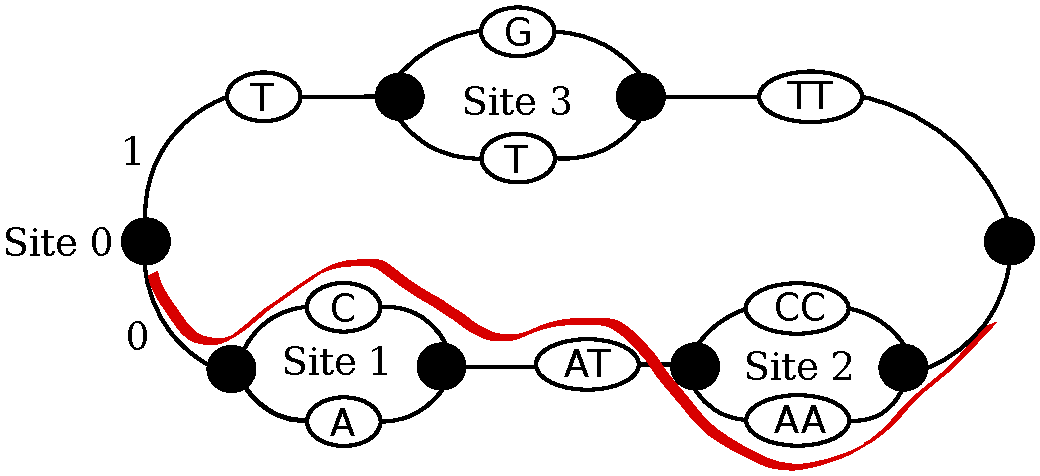
\includegraphics{img/example_graph.pdf}
\caption{Genome graph with haploid genotyped sample as red path
\label{toy_graph}}
\end{figure}

In Figure \ref{toy_graph}, black nodes mark site entry and exit points.
Each variant site is labeled by a unique positive integer ID, and each
outgoing branch from the start of a variant site is labeled by a unique
positive integer, called its \textbf{haplogroup}.

Assume the ploidy is 1, and we are genotyping a sample whose genotyped
path in the graph is the red line. The jVCF of this genotyped sample
would look like this:

\newpage

\begin{center}\rule{0.5\linewidth}{0.5pt}\end{center}

\begin{verbatim}
{
  "Sites":[
    {"ALS":["AATAA","CATAA"],"FT":[[]],"GT":[[1]],"HAPG":[[0]],"POS":1,"SEG":"myRef"},
    {"ALS":["A","C"],"FT":[[]],"GT":[[1]],"HAPG":[[1]],"POS":1,"SEG":"myRef"},
    {"ALS":["AA"],"FT":[[]],"GT":[[0]],"HAPG":[[0]],"POS":4,"SEG":"myRef"},
    {"ALS":["T"],"FT":[[]],"GT":[[null]],"HAPG":[[]],"POS":2,"SEG":"myRef"}
  ],
  "Site_Fields": {
    "ALS": {
      "Desc": "Alleles at this site"
    },
    "FT": {
      "Desc": "Filters failed in a sample"
    },
    "GT": {
      "Desc": "Genotype"
    },
    "HAPG": {
      "Desc": "Sample haplogroups of genotyped alleles"
    },
    "POS": {
      "Desc": "Position on reference or pseudo-reference"
    },
    "SEG": {
      "Desc": "Segment ID"
    }
  },
  "Samples": [
    {
      "Desc": "mySample description",
      "Name": "mySample"
    }
  ],
  "Filters": {
    "MINQ": {
      "Desc": "Call is below minimum quality"
    }
  },
  "Model": "myGenotypingModel",
  "Child_Map": {
    "0": {
      "0": [1,2],
      "1": [3]
    }
  },
  "Lvl1_Sites": [0]
}
\end{verbatim}

\begin{center}\rule{0.5\linewidth}{0.5pt}\end{center}

\newpage

\hypertarget{specification}{%
\section{Specification}\label{specification}}

There are 7 required keys in jVCF, which can appear in any order. We
list each of the required keys below, giving for each the type and
description of its corresponding value.

Extra keys beyond these can be used.

\hypertarget{sites}{%
\subsection{Sites}\label{sites}}

\begin{description}
\item[Type]
Array
\item[Description]
Each element is a Site object
\end{description}

\hypertarget{site_obj}{%
\subsubsection{Site objects}\label{site_obj}}

A Site object is like a data line in the VCF format. It describes
variant calls at one site. The following keys are required:

\begin{longtable}[]{@{}cc@{}}
\toprule
\begin{minipage}[b]{0.16\columnwidth}\centering
Key\strut
\end{minipage} & \begin{minipage}[b]{0.64\columnwidth}\centering
Value Type\strut
\end{minipage}\tabularnewline
\midrule
\endhead
\begin{minipage}[t]{0.16\columnwidth}\centering
ALS\strut
\end{minipage} & \begin{minipage}[t]{0.64\columnwidth}\centering
Array of strings\strut
\end{minipage}\tabularnewline
\begin{minipage}[t]{0.16\columnwidth}\centering
SEG\strut
\end{minipage} & \begin{minipage}[t]{0.64\columnwidth}\centering
String\strut
\end{minipage}\tabularnewline
\begin{minipage}[t]{0.16\columnwidth}\centering
POS\strut
\end{minipage} & \begin{minipage}[t]{0.64\columnwidth}\centering
Number\strut
\end{minipage}\tabularnewline
\begin{minipage}[t]{0.16\columnwidth}\centering
GT\strut
\end{minipage} & \begin{minipage}[t]{0.64\columnwidth}\centering
Array of array of numbers, `null' or empty\strut
\end{minipage}\tabularnewline
\begin{minipage}[t]{0.16\columnwidth}\centering
HAPG\strut
\end{minipage} & \begin{minipage}[t]{0.64\columnwidth}\centering
Array of array of numbers or empty\strut
\end{minipage}\tabularnewline
\begin{minipage}[t]{0.16\columnwidth}\centering
FT\strut
\end{minipage} & \begin{minipage}[t]{0.64\columnwidth}\centering
Array of arrays of strings or empty\strut
\end{minipage}\tabularnewline
\bottomrule
\end{longtable}

Here is a more detailed explanation of the keys:

\begin{itemize}
\item
  \texttt{ALS}: does not need to store all possible alleles at the
  variant site. It must store at least one allele which is the
  `reference' for this site. The reference allele must be the allele
  obtained by following haplogroup 0 from the start of the site to the
  end of the site. All called alleles should also be present in
  \texttt{ALS}.
\item
  \texttt{SEG}: the name of the genomic segment the site lies on,
  e.g.~chromosome or the name of a reference genome.
\item
  \texttt{POS}: 1-based position, offset from the last non-nested site
  (see \protect\hyperlink{lvl1_sites}{Lvl1\_Sites}). The position of
  sites contained in other sites is expressed relative to the reference
  path through the containing site, which is obtained by following
  haplogroup 0.
\item
  \texttt{GT} and \texttt{HAPG}: are arrays of arrays. The two array
  levels are:

  \begin{enumerate}
  \def\labelenumi{\arabic{enumi}.}
  \tightlist
  \item
    Samples. This should have the same size as the array in
    \protect\hyperlink{samples}{Samples}.
  \item
    Ploidy. This should have one entry per chromosome copy, or
    chromosome population (eg tumour subclones or mixed infections).
  \end{enumerate}

  For example, to access the first sample's genotype calls at a site,
  you access the 0th element of the \texttt{GT} array. If you have a
  diploid genotyped sample, the first and second chromosome calls are
  the 0th and 1st elements of that array.
\item
  \texttt{FT}: also an array of arrays. The first level is the samples,
  and the second the filters set for that sample.
\end{itemize}

You can, of course, use more keys. For each used key,
\protect\hyperlink{site_fields}{Site\_Fields} needs to provide a
description of its meaning. The required keys here must be present in
\protect\hyperlink{site_fields}{Site\_Fields}.

\hypertarget{site_fields}{%
\subsection{Site\_Fields}\label{site_fields}}

\begin{description}
\item[Type]
Object
\item[Description]
Each entry describes the fields that can appear in
\protect\hyperlink{site_obj}{Site objects}.
\end{description}

For each key which appears in \protect\hyperlink{site_obj}{Site
objects}, a corresponding key must be present here. The following keys
are required to be present:

\begin{longtable}[]{@{}cc@{}}
\toprule
\begin{minipage}[b]{0.16\columnwidth}\centering
Key\strut
\end{minipage} & \begin{minipage}[b]{0.64\columnwidth}\centering
Meaning\strut
\end{minipage}\tabularnewline
\midrule
\endhead
\begin{minipage}[t]{0.16\columnwidth}\centering
ALS\strut
\end{minipage} & \begin{minipage}[t]{0.64\columnwidth}\centering
Genotyped alleles at this site\strut
\end{minipage}\tabularnewline
\begin{minipage}[t]{0.16\columnwidth}\centering
SEG\strut
\end{minipage} & \begin{minipage}[t]{0.64\columnwidth}\centering
Segment (eg chromosome) on which the site lies\strut
\end{minipage}\tabularnewline
\begin{minipage}[t]{0.16\columnwidth}\centering
POS\strut
\end{minipage} & \begin{minipage}[t]{0.64\columnwidth}\centering
1-based position relative to haplogroup reference\strut
\end{minipage}\tabularnewline
\begin{minipage}[t]{0.16\columnwidth}\centering
GT\strut
\end{minipage} & \begin{minipage}[t]{0.64\columnwidth}\centering
Genotype calls\strut
\end{minipage}\tabularnewline
\begin{minipage}[t]{0.16\columnwidth}\centering
HAPG\strut
\end{minipage} & \begin{minipage}[t]{0.64\columnwidth}\centering
Haplogroup calls: haplogroup the called allele(s) lie on\strut
\end{minipage}\tabularnewline
\begin{minipage}[t]{0.16\columnwidth}\centering
FT\strut
\end{minipage} & \begin{minipage}[t]{0.64\columnwidth}\centering
Filters set\strut
\end{minipage}\tabularnewline
\bottomrule
\end{longtable}

Each key corresponds to an object with at least a ``Desc'' key which
gives a description of the field.

\hypertarget{samples}{%
\subsection{Samples}\label{samples}}

\begin{description}
\item[Type]
Array
\item[Description]
Each entry is an object describing one genotyped sample.
\end{description}

Each entry must contain the following keys: ``Name'' and ``Desc'',
giving the sample name and its description. The order of the samples
matters: it must match that in \protect\hyperlink{site_obj}{Site
objects}.

\hypertarget{filters}{%
\subsection{Filters}\label{filters}}

\begin{description}
\item[Type]
Object
\item[Description]
Describes the filters that can appear in Site objects.
\end{description}

Each filter that appears under the ``FT'' key in
\protect\hyperlink{site_obj}{Site objects} must be described here. Each
key gives the filter name and each value is an object with at least a
``Desc'' key giving the filter's description.

\hypertarget{model}{%
\subsection{Model}\label{model}}

\begin{description}
\item[Type]
String
\item[Description]
The name, or a description, of the genotyping model that was used.
\end{description}

\hypertarget{child_map}{%
\subsection{Child\_Map}\label{child_map}}

\begin{description}
\item[Type]
Object
\item[Description]
Records parent/site relationships between variant sites and on which
haplogroups child sites lie.
\end{description}

Each key corresponds to a site index in the
\protect\hyperlink{sites}{Sites} array. The value associated to each key
is a Child listing object.

Starting from each entry of the
\protect\hyperlink{lvl1_sites}{Lvl1\_Sites}, the Child\_Map can be
recursively traversed to recover the full parent/child site structure of
the graph.

\hypertarget{child-listing}{%
\subsubsection{Child listing}\label{child-listing}}

A Child listing is an object whose keys are haplogroups and whose values
are arrays of site indices. It records, for a given parent site, what
child sites it has, and which haplogroups the child sites fall under.

\hypertarget{lvl1_sites}{%
\subsection{Lvl1\_Sites}\label{lvl1_sites}}

\begin{description}
\item[Type]
Array
\item[Description]
Lists the indices of sites which are not nested in others.
\end{description}

Each element of this array corresponds to a site which has no parents;
the value is the index at which to access this site in the
\protect\hyperlink{sites}{Sites} array.

Each site referred to in this array may or may not have children,
depending on whether or not it appears in
\protect\hyperlink{child_map}{Child\_Map}.
